% IEEE TNSM manuscript
\documentclass[journal]{IEEEtran}

\usepackage{cite}
\usepackage{amsmath,amssymb,amsfonts}
\usepackage{graphicx}
\usepackage{booktabs}
\usepackage{tabularx}
\usepackage{textcomp}
\usepackage{xcolor}
\usepackage{tikz}
\usepackage{url}
\usepackage{hyperref}
\usetikzlibrary{positioning,arrows.meta,calc,fit,backgrounds}

\definecolor{PrismBlue}{HTML}{1F4E79}
\definecolor{PrismLightBlue}{HTML}{EDF5FB}
\definecolor{PrismOrange}{HTML}{C45C26}
\definecolor{PrismGreen}{HTML}{2F6F4E}
\definecolor{PrismLightGreen}{HTML}{EAF6EF}
\definecolor{PrismGray}{HTML}{5A5A5A}

\hypersetup{hidelinks}

\begin{document}

\title{Telemetry-Aware Risk-Sensitive Ranking for Intervention Service Management in AIoT\thanks{Alternate title under consideration: Risk-Sensitive Ranking for Managed AIoT Intervention Services under Unreliable Telemetry.}}

\author{Alema Emran}

\maketitle

%--------------------------------------------------------------------------
\begin{abstract}
Closed-loop AIoT intervention services must rank prompts while context beliefs are degraded by independent and bursty packet loss as well as sensor ambiguity.
Many managed pipelines collapse the belief to a MAP label before ranking; it is unclear whether richer uncertainty representations help an explicit ranking module as monitoring reliability worsens.
We isolate ranking inside a fixed Sense--Monitor--Plan--Rank--Safety--Deliver loop on StepCountJITAI, hold candidates and one-step utility fixed and stress the monitor with a noise proxy \(\sigma\) plus matched-mean independent and Gilbert--Elliott packet-loss channels.
Across matched operators (30 seeds), richer risk-neutral uncertainty representations alone do not outperform MAP---in contrast to soft-belief gains reported for learned RL policies on the same family of simulators.
CVaR reduces high-\(\sigma\) regret by \(24.89\) units at \(\sigma=2\), while the Hybrid gate (\(\pi^\star=0.7\)) reduces it by \(26.09\) (bootstrap \(95\%\) CIs exclude zero); both gains persist on \(\alpha\times p_{\mathrm{loss}}\) heatmaps at \(\sigma\in\{1,2\}\) and reverse when habituation / disengagement is frozen, consistent with trajectory mediation.
We also report a deployable specialised-prompt / SLA-proxy KPI and multi-tenant ranking latency under SLA-style targets (up to \(64\) concurrent users).
\end{abstract}

\begin{IEEEkeywords}
Network and service management, unreliable telemetry, packet loss, closed-loop AIoT, intervention ranking, CVaR, SLA, policy regret
\end{IEEEkeywords}

%--------------------------------------------------------------------------
\section{Introduction}
\label{sec:introduction}

Physical-activity and wellbeing support increasingly runs as a closed-loop managed service on wearables and edge gateways: the system senses behaviour, maintains a belief about the user's situation and delivers a short prompt when help is most useful~\cite{nahum2018jitai,liao2020heartsteps}.
From a network and service management perspective, the ranking stage is a swappable decision module inside that service loop: it consumes monitored belief state and returns an intervention action under latency and reliability constraints typical of edge delivery~\cite{shi2016edge,borsatti2024kubetwin}.
The monitoring path is itself networked telemetry: missing packets, transport gaps and jitter flatten the context belief in the same way that abstract inference noise does, so ranking under partial observability is also a problem of deciding under unreliable telemetry~\cite{wang2023dtservice}.
Getting that choice wrong is costly in service terms.
A poorly timed or poorly matched prompt raises habituation and disengagement; after repeated misses the prompts feel like noise and the managed service that looked complete on a demo day quietly fails in daily use~\cite{nahum2018jitai,karine2024stepcount}.
Reliable ranking under degraded monitoring is therefore a practical requirement for managed AIoT intervention services.

The root difficulty is that the platform never sees why a prompt would help.
It maintains a belief over latent context from noisy steps, missing packets and ambiguous behaviour~\cite{kaelbling1998pomdp}.
When that belief is sharp, collapsing it to a MAP label before ranking is often enough.
When the belief is flat---whether from sensor ambiguity or degraded telemetry---the same rule can select a specialised prompt that is strong in one situation and weak in the other and the mistake compounds over the episode.

Modern pipelines already implement a modular loop---sense, monitor, plan, rank, safety, deliver~\cite{yao2023react,shi2016edge,wang2023dtservice}---yet many still collapse belief before ranking.
Soft belief has been shown to help trained RL policies under context inference error~\cite{karine2023uai}, but modular managed systems expose a ranking module rather than an end-to-end policy~\cite{sutton2018rl}.
What that module should consume as telemetry reliability worsens remains unclear.

This paper isolates ranking inside a fixed modular closed-loop AIoT service on StepCountJITAI~\cite{karine2024stepcount,towers2024gymnasium}.
We use \emph{agentic} only in that narrow, pre-LLM sense: a bounded Sense--Monitor--Plan--Rank--Safety--Deliver loop with no autonomous tool use or multi-step language planning.
The contribution is not a new simulator and not a new CVaR algorithm: it is a controlled comparison of uncertainty representations inside an explicit ranking module under matched candidates, matched one-step utilities and degraded monitoring---including a negative result for risk-neutral soft belief / LTR relative to MAP, which does not contradict soft-belief gains for trained RL policies~\cite{karine2023uai}.
We sweep a noise parameter \(\sigma\) as a monitoring-reliability proxy, add explicit packet-loss channels and compare operators by mean per-step policy regret.
The primary scientific story is risk-sensitive ranking under that reliability stress: after a risk-neutral regime map shows that richer belief features alone do not beat MAP, we change the aggregation rule to CVaR / Hybrid and analyse when and why that helps.
The main contributions are as follows.
\begin{itemize}
  \item \textbf{Isolated ranking comparison.} We fix \(\rho:(p_t,x_t,\mathcal{A})\mapsto a_t\) so that only the uncertainty representation inside ranking changes inside an otherwise fixed managed service loop.
  \item \textbf{Risk-neutral regime map (30 seeds).} Across six operators over \(\sigma\in\{0,0.4,1.0,2.0\}\), soft belief and LTR do not automatically beat MAP; BASR is significantly worse.
  \item \textbf{Risk-sensitive aggregation under telemetry impairment.} \(\mathrm{CVaR}_\alpha\) cuts high-\(\sigma\) regret by \(24.89\) units at \(\sigma=2\) (\(\approx 49\%\) relative); the Hybrid gate at operational \(\pi^\star=0.7\) cuts it by \(26.09\) (paired bootstrap CIs exclude zero). Gains persist under stochastic / process-noise locks and on matched-mean independent / Gilbert--Elliott \(\alpha\times p_{\mathrm{loss}}\) heatmaps at \(\sigma\in\{1,2\}\).
  \item \textbf{Trajectory-mediated mechanism.} A one-step twin recovers \(\pi^\star\) as a decision rule but not the episode regret win; freezing habituation / disengagement reverses the CVaR advantage.
  \item \textbf{Service-facing evidence.} A deployable specialised-prompt / SLA proxy, \(\pi^\star\) sweep versus reward/regret and multi-tenant ranking latency under SLA-style targets.
\end{itemize}

The remainder of this paper is organized as follows.
Section~\ref{sec:related} reviews related work.
Section~\ref{sec:system-model} develops the system model and problem.
Section~\ref{sec:direction} describes the experimental methodology.
Section~\ref{sec:results} reports results.
Section~\ref{sec:discussion} discusses interpretation and limitations.
Section~\ref{sec:conclusion} concludes.

%--------------------------------------------------------------------------
\section{Related Work}
\label{sec:related}

\subsection{Decision Making under Partial Observability}
Classical POMDPs formalise acting under a belief over latent state~\cite{kaelbling1998pomdp}; practical systems rely on approximate belief tracking rather than exact solutions~\cite{pineau2003point}.
In mobile health, JITAIs personalise prompts from streaming data~\cite{nahum2018jitai,liao2020heartsteps,tewari2017bandits}.
Karine et~al.\ showed that context inference error degrades JITAI policies and that soft context probabilities help trained RL methods as error grows~\cite{karine2023uai}; StepCountJITAI provides a controllable simulator for that setting~\cite{karine2024stepcount,towers2024gymnasium}.
That soft-belief evidence is for learned policies, not for an explicit ranking rule under a fixed one-step utility.

\subsection{Ranking under Uncertainty}
Learning-to-rank supplies listwise scorers for small candidate sets~\cite{burges2010lambdamart,liu2009ltr,ke2017lightgbm}.
Selective prediction adds abstention under low confidence~\cite{elyaniv2010selective,geifman2017selective}.
Risk-aware and safe recommendation lines argue that mean-utility ranking can be insufficient when downside outcomes matter~\cite{garcia2015saferl}, yet controlled comparisons of uncertainty representations inside a matched JITAI ranking interface remain scarce.

\subsection{Risk-Sensitive and Robust Sequential Decisions}
Conditional value-at-risk provides a coherent tail-sensitive criterion~\cite{rockafellar2000cvar,chow2015cvar}.
Distributional RL models return distributions rather than expectations~\cite{bellemare2017distributional,dabney2018qr} and robust MDP formulations guard against adversarial transition uncertainty~\cite{nilim2005robust,iyengar2005robust}.
Safe RL surveys related constraints on harmful behaviour~\cite{garcia2015saferl}.
We use CVaR as an aggregation rule over belief-conditioned one-step utilities inside ranking, not as a new distributional or robust-MDP algorithm.

\subsection{Modular Pipelines and Managed Service Modules}
Network and service management increasingly studies digital-twin-assisted orchestration and closed-loop automation for softwarized infrastructures~\cite{borsatti2024kubetwin,wang2023dtservice}.
KubeTwin uses a twin to evaluate deployment and management policies for large Kubernetes applications without disturbing the live continuum~\cite{borsatti2024kubetwin}; twin-driven self-healing similarly predicts performance and redeploys services away from degraded edge nodes and links~\cite{wang2023dtservice}.
Our setting is narrower but aligned: we keep a digital twin of the intervention loop (StepCountJITAI) and treat the ranking stage as the swappable AI decision module under degraded monitoring, analogous to swapping a managed policy while Sense--Monitor--Plan--Safety--Deliver stay fixed around Rank.
That modularity is the same idea as intent-based / closed-loop automation in softwarized networks~\cite{clemm2022ibn,boutaba2018mlnet}: a management intent is realised by a replaceable decision module rather than by rewriting the whole pipeline.
Risk-sensitive decision-making already uses tail criteria when mean utility hides downside outcomes~\cite{garcia2015saferl}; we ask the analogous question for intervention ranking when the impairment is unreliable monitoring rather than only sensor noise.
Modular and edge loops already separate those stages~\cite{yao2023react,shi2016edge}; we use that scaffolding and vary only ranking under abstract \(\sigma\) plus explicit independent and Gilbert--Elliott bursty packet-loss channels~\cite{gilbert1960capacity,elliott1963estimates} that stale the belief delivered to the ranker.
Matched mean loss is enough for the claim we make---whether risk-sensitive ranking remains preferable as monitoring drops increase---without fitting a radio or MQTT delay trace.
The gap we target is therefore service-relevant: under matched candidates, matched utilities and degraded telemetry proxies, how should uncertainty enter ranking and when does changing aggregation improve closed-loop outcomes?

%--------------------------------------------------------------------------
\section{System Model and Problem Formulation}
\label{sec:system-model}

\subsection{Overview of the Closed-Loop AIoT Service}
\label{sec:loop}

We consider a closed-loop AIoT system that repeatedly senses, decides and acts on behalf of one user.
The loop has six stages, shown in Fig.~\ref{fig:architecture}.
A wearable or edge node first publishes telemetry over a lightweight message transport.
Monitoring then converts that telemetry into a belief over the latent context together with a vector of behavioural state features and planning enumerates a fixed set of candidate interventions.
The ranking stage scores those candidates and returns a single action, after which a safety stage checks it against an allow-list before delivery.
Throughout the study we vary only the ranking stage and hold every other stage fixed.
The orchestration and transport layers are treated as deployment context, not as a claimed contribution.

\begin{figure*}[!t]
\centering
\resizebox{\textwidth}{!}{%
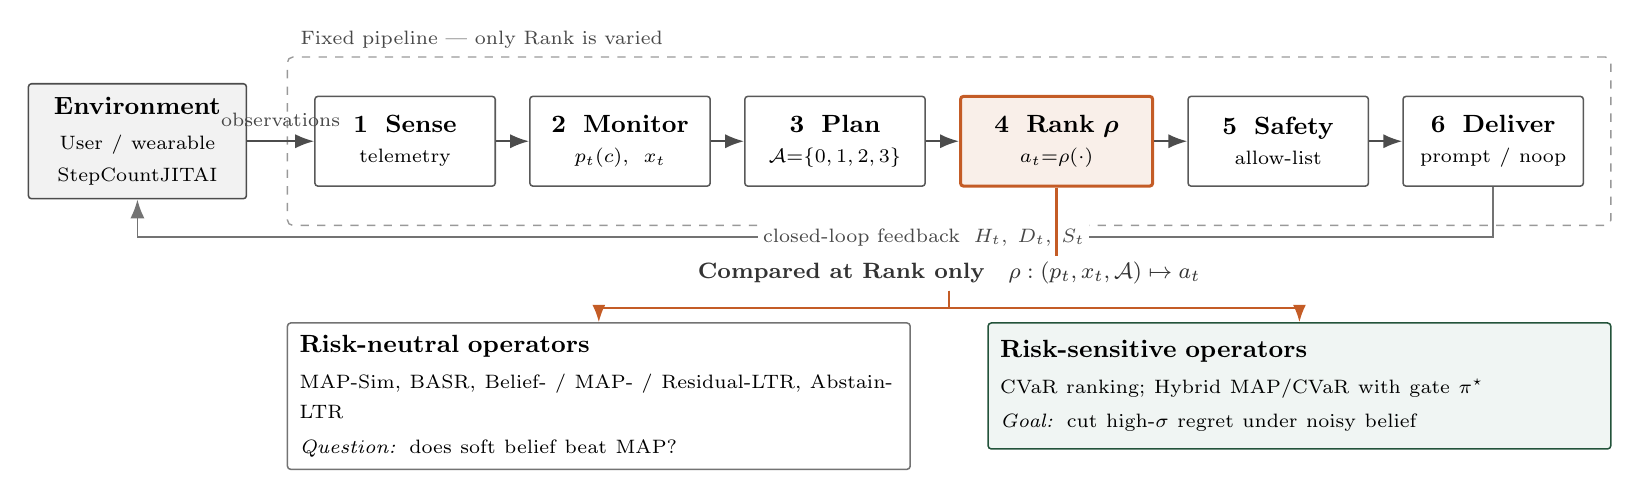
\begin{tikzpicture}[
  font=\small,
  >=Latex,
  every node/.style={align=center},
  arr/.style={-{Latex[length=2.4mm]}, line width=0.7pt, draw=black!70},
  fbarr/.style={-{Latex[length=2.4mm]}, line width=0.65pt, draw=black!55},
  stage/.style={
    rounded corners=1.1pt, draw=black!65, fill=white,
    minimum height=11.4mm, text width=21.5mm,
    inner sep=2pt, line width=0.55pt
  },
  env/.style={
    rounded corners=1.1pt, draw=black!70, fill=black!5,
    minimum height=14.6mm, text width=26mm,
    inner sep=2.4pt, line width=0.55pt
  },
  rankbox/.style={
    rounded corners=1.1pt, draw=PrismOrange, fill=PrismOrange!10,
    minimum height=11.4mm, text width=23mm,
    inner sep=2pt, line width=1.1pt
  },
  card/.style={
    rounded corners=1.2pt, align=left,
    text width=76mm, minimum height=16mm,
    inner sep=4.4pt, line width=0.55pt
  },
  note/.style={font=\scriptsize, text=black!72},
]
\node[env] (E) {%
  \textbf{Environment}\\[1.5pt]
  {\scriptsize User / wearable}\\[0.4pt]
  {\scriptsize StepCountJITAI}
};
\node[stage, right=8.5mm of E] (S1)
  {\textbf{1~~Sense}\\[-0.2pt]{\scriptsize telemetry}};
\node[stage, right=4.2mm of S1] (S2)
  {\textbf{2~~Monitor}\\[-0.2pt]{\scriptsize $p_t(c),\;x_t$}};
\node[stage, right=4.2mm of S2] (S3)
  {\textbf{3~~Plan}\\[-0.2pt]{\scriptsize $\mathcal{A}{=}\{0,1,2,3\}$}};
\node[rankbox, right=4.2mm of S3] (S4)
  {\textbf{4~~Rank $\boldsymbol{\rho}$}\\[-0.2pt]{\scriptsize $a_t{=}\rho(\cdot)$}};
\node[stage, right=4.2mm of S4] (S5)
  {\textbf{5~~Safety}\\[-0.2pt]{\scriptsize allow-list}};
\node[stage, right=4.2mm of S5] (S6)
  {\textbf{6~~Deliver}\\[-0.2pt]{\scriptsize prompt / noop}};

\begin{scope}[on background layer]
\node[draw=black!40, dashed, rounded corners=2pt,
      inner xsep=3.4mm, inner ysep=4.8mm,
      fit=(S1)(S2)(S3)(S4)(S5)(S6), line width=0.5pt] (AF) {};
\end{scope}
\node[note, anchor=south west, fill=white, inner sep=1.4pt]
  at ([xshift=1.2mm,yshift=0.4mm]AF.north west)
  {Fixed pipeline --- only Rank is varied};

\draw[arr] (E.east) -- node[note, above=1.5pt]{observations} (S1.west);
\foreach \u/\v in {S1/S2,S2/S3,S3/S4,S4/S5,S5/S6}
  \draw[arr] (\u) -- (\v);

\coordinate (fb) at ([yshift=-6.4mm]S6.south);
\draw[fbarr] (S6.south) -- (S6.south |- fb) -| (E.south);
\node[note, fill=white, inner sep=1.8pt]
  at ($(S6.south |- fb)!0.42!(E.south |- fb)$)
  {closed-loop feedback $\;H_t,\;D_t,\;S_t$};

\node[card, draw=black!55, fill=white,
      below=12.2mm of AF.south west, anchor=north west] (P1) {%
  \textbf{Risk-neutral operators}\\[2pt]
  {\scriptsize MAP-Sim, BASR, Belief- / MAP- / Residual-LTR, Abstain-LTR}\\[1.5pt]
  {\scriptsize\textit{Question:} does soft belief beat MAP?}
};
\node[card, draw=PrismGreen!75!black, fill=PrismGreen!7,
      below=12.2mm of AF.south east, anchor=north east] (P2) {%
  \textbf{Risk-sensitive operators}\\[2pt]
  {\scriptsize CVaR ranking; Hybrid MAP/CVaR with gate $\pi^\star$}\\[1.5pt]
  {\scriptsize\textit{Goal:} cut high-$\sigma$ regret under noisy belief}
};

\node[font=\footnotesize, text=black!80, fill=white, inner sep=2pt]
  (CTITLE) at ([yshift=6.2mm]$(P1.north)!0.5!(P2.north)$)
  {\textbf{Compared at Rank only}\quad
   $\rho:(p_t,x_t,\mathcal{A})\mapsto a_t$};

\draw[PrismOrange, line width=0.85pt] (S4.south) -- (S4.south |- CTITLE.north);
\draw[PrismOrange, line width=0.7pt, -{Latex[length=2.2mm]}]
  (CTITLE.south) -- ++(0,-2.2mm) -| (P1.north);
\draw[PrismOrange, line width=0.7pt, -{Latex[length=2.2mm]}]
  (CTITLE.south) -- ++(0,-2.2mm) -| (P2.north);
\end{tikzpicture}%
}
\caption{Closed-loop modular architecture for intervention delivery on StepCountJITAI.
The dashed frame is held fixed.
Orange marks the ranking module \(\rho\), the only stage varied.
Green marks the risk-sensitive operators studied after the risk-neutral regime map.}
\label{fig:architecture}
\end{figure*}

\subsection{Environment and State Variables}
\label{sec:environment}

We adopt StepCountJITAI as the world model because it exposes an explicit context noise parameter and standard environment semantics~\cite{karine2024stepcount,towers2024gymnasium}.
Time is discrete and indexed by \(t=1,\dots,T\), where one step corresponds to one intervention decision opportunity.
At step \(t\) the environment holds a latent context \(c_t\in\mathcal{C}=\{0,1\}\), which encodes the behavioural situation that determines which prompt is effective.
It also tracks a habituation level \(H_t\in[0,1]\), a disengagement risk \(D_t\in[0,1]\) and a step-count state \(S_t\ge 0\).
Habituation rises when prompts are delivered repeatedly and reduces their effect; disengagement risk rises when prompts are poorly matched and reduces future responsiveness.
The reward \(R_t\in\mathbb{R}\) is the step-count contribution realized after the chosen action.
Table~\ref{tab:notation} summarizes the notation used throughout.

\begin{table}[t]
\centering
\caption{Notation used in the system model.}
\label{tab:notation}
\footnotesize
\begin{tabular}{@{}ll@{}}
\toprule
Symbol & Meaning \\
\midrule
\(t,\,T\) & decision step index and episode horizon \\
\(c_t\in\mathcal{C}\) & latent true context, \(\mathcal{C}=\{0,1\}\) \\
\(\sigma\ge 0\) & context inference noise level \\
\(p_t(c)\) & belief that the context equals \(c\) at step \(t\) \\
\(\hat{c}_t\) & collapsed context, \(\hat{c}_t=\arg\max_c p_t(c)\) \\
\(\pi_t\) & belief peak, \(\pi_t=\max_c p_t(c)\) \\
\(H_t,\,D_t,\,S_t\) & habituation, disengagement risk, step-count state \\
\(x_t\in\mathbb{R}^{7}\) & feature vector exposed to the ranking module \\
\(\mathcal{A}\) & candidate action set, \(|\mathcal{A}|=4\) \\
\(a_t\) & action selected by the ranking operator \\
\(U_t(a\mid c)\) & one-step counterfactual utility of \(a\) assuming context \(c\) \\
\(U_t^\star(a)\) & oracle utility, evaluated at the true context \(c_t\) \\
\(a_t^\star\) & oracle-best action at step \(t\) \\
\(R_t\) & realized environment reward at step \(t\) \\
\(\rho\) & ranking operator, \(a_t=\rho(p_t,x_t,\mathcal{A})\) \\
\(f_\theta\) & learned ranking score with parameters \(\theta\) \\
\(\tau\) & confidence threshold for deferral \\
\(\alpha\) & tail level of the risk-sensitive aggregation \\
\(H,\,M,\,L\) & matched, robust and mismatched utility levels \\
\(\pi^\star\) & belief-peak threshold of the hybrid gate (operational \(0.7\)) \\
\(p_{\mathrm{loss}}\) & mean monitoring packet-loss probability \\
\bottomrule
\end{tabular}
\end{table}

\subsection{Candidate Interventions}
\label{sec:actions}

The planning stage exposes a fixed candidate set at every decision step,
\begin{align}
\label{eq:actions}
\mathcal{A}=\{0,1,2,3\}\:,
\end{align}
where action \(0\) delivers no prompt, action \(1\) delivers a low-intensity prompt that is useful in either context and actions \(2\) and \(3\) deliver context-specialized prompts.
The specialized prompts are the source of difficulty because each one is strong in one context and weak in the other.
The candidate set is fixed so that any performance difference is attributable to the ranking rule alone.

\subsection{Observation Model and Belief}
\label{sec:belief}

The ranking module never observes \(c_t\).
The monitoring stage supplies a belief
\begin{align}
\label{eq:belief}
p_t(c)=\Pr\!\left(c_t=c \mid o_{1:t}\right)\:,
\end{align}
where \(o_{1:t}\) denotes the observation history.
The noise level \(\sigma\) controls how informative that history is, so a larger \(\sigma\) flattens the belief and increases inference error.
In this paper we treat \(\sigma\) as a controllable \emph{monitoring-reliability proxy}: larger \(\sigma\) stands in for regimes in which telemetry is less informative because of sensor ambiguity and/or networked degradation (loss, gaps, jitter).
To make the networked reading explicit for TNSM, we also impair the monitoring path with two packet-loss channels that share the same mean loss rate \(p_{\mathrm{loss}}\):
\begin{itemize}
  \item \textbf{Independent loss:} each monitoring packet is dropped independently with probability \(p_{\mathrm{loss}}\) (Bernoulli).
  \item \textbf{Bursty loss:} a Gilbert--Elliott two-state Markov channel~\cite{gilbert1960capacity,elliott1963estimates} with a lossless Good state and an always-loss Bad state, mean burst length \(3\) steps and steady-state \(\Pr(\mathrm{Bad})=p_{\mathrm{loss}}\).
\end{itemize}
On a drop the environment continues to evolve, but the ranking module consumes the last successfully delivered belief (stale monitoring).
Matching the two channels on mean \(p_{\mathrm{loss}}\) isolates the effect of loss clustering: any remaining gap is burstiness, not a higher average drop rate.
We do not fit a physical radio or MQTT delay model; the channels are controllable service-management stresses for ranking under degraded monitoring.
The module also receives the feature vector
\begin{align}
\label{eq:features}
x_t=\big(p_t(0),\,p_t(1),\,\hat{c}_t,\,H_t,\,D_t,\,S_t,\,t\big)\:,
\end{align}
where \(\hat{c}_t=\arg\max_{c} p_t(c)\) is the collapsed context.
Uncertainty can therefore enter a ranking rule in two ways, either as explicit features in \(x_t\) or as a distribution over simulated outcomes.

\subsection{Utility Model and Oracle}
\label{sec:utility}

Each candidate needs a score.
We use the one-step counterfactual utility obtained by querying the simulator under an assumed context:
\begin{align}
\label{eq:utility}
U_t(a\mid c)=R\big(\mathrm{step}(a;\,c)\big)\:,
\end{align}
where the state is snapshotted, the context is set to \(c\), the action \(a\) is applied, the reward is recorded and the state is restored.
Every operator therefore has access to the same simulator and the same computational primitive.
The oracle evaluates the same quantity at the true context,
\begin{align}
\label{eq:oracle}
U_t^\star(a)=U_t(a\mid c_t)\:,
\end{align}
and the oracle-best action is
\begin{align}
\label{eq:bestaction}
a_t^\star=\arg\max_{a\in\mathcal{A}} U_t^\star(a)\:.
\end{align}
The oracle is used only for evaluation; it is never available to any ranking operator.

\subsection{Ranking Interface}
\label{sec:interface}

A ranking operator is a map
\begin{align}
\label{eq:operator}
\rho:\;\big(p_t,\,x_t,\,\mathcal{A}\big)\;\mapsto\;a_t\in\mathcal{A}\:,
\end{align}
and the six operators studied here differ only in how \(p_t\) is used.
Table~\ref{tab:operators} summarizes the operators and their decision rules.
Belief collapse simulates a single context, belief averaging integrates over the belief and the learned operators score candidates from features.
The deferral operator combines a learned score with a fallback, using a confidence signal derived from the normalized belief entropy and the margin between the top two scores, with threshold \(\tau=0.45\) selected on a separate validation grid.

\begin{table}[t]
\centering
\caption{Ranking operators compared under the same interface.}
\label{tab:operators}
\footnotesize
\begin{tabular}{@{}lp{4.55cm}@{}}
\toprule
Operator & Decision rule \\
\midrule
MAP-Sim & \(a_t=\arg\max_a U_t(a\mid\hat{c}_t)\) \\
BASR & \(a_t=\arg\max_a \mathbb{E}_{c\sim p_t}\!\big[U_t(a\mid c)\big]\) \\
Belief-LTR & \(a_t=\arg\max_a f_\theta(x_t,a)\), full \(x_t\) \\
MAP-LTR & \(a_t=\arg\max_a f_\theta(x_t,a)\), belief entries removed \\
Residual-LTR & \(a_t=\arg\max_a \big[U_t(a\mid\hat{c}_t)+\delta_\theta(x_t,a)\big]\) \\
Abstain-LTR & Belief-LTR if confidence \(\ge\tau\), else MAP-Sim \\
Oracle & \(a_t=a_t^\star\), evaluation upper bound only \\
\bottomrule
\end{tabular}
\end{table}

\subsection{Assumptions}
\label{sec:assumptions}

The system model rests on five assumptions that bound the scope of the conclusions.
The candidate set is fixed and small, so ranking is a selection problem rather than a generation problem.
The ranking score is a one-step counterfactual utility, which makes the operators myopic by construction and prevents planning over the horizon.
The belief supplied by the monitoring stage is treated as given: belief estimation quality is controlled through \(\sigma\) rather than modelled separately.
The locked evaluation uses the deterministic dynamics setting of the environment for the risk-neutral regime map, removing transition noise as a confound and isolating context uncertainty; stochastic dynamics and process-noise transfer are reported separately for the risk-sensitive operators.
Finally, primary evaluation is simulation-based; no clinical efficacy claim is made and no human subject data are used.
A secondary lab ESP32 / MQTT loop is reported only as deployment feasibility (connectivity and ranking-stage timing), not as a substitute for the StepCountJITAI regret study.

\subsection{Problem Statement}
\label{sec:problem}

Let \(a_t=\rho(p_t,x_t,\mathcal{A})\) be the action chosen by operator \(\rho\).
The quality of that choice is measured by the mean per-step policy regret against the oracle,
\begin{align}
\label{eq:regret}
\mathcal{R}(\rho)=\frac{1}{T}\sum_{t=1}^{T}\Big(U_t^\star(a_t^\star)-U_t^\star(a_t)\Big)\:,
\end{align}
which is zero when the operator always selects an oracle-best action.
The research question follows directly: given the interface in~\eqref{eq:operator} and the utility in~\eqref{eq:utility}, which representation of \(p_t\) inside \(\rho\) minimizes \(\mathcal{R}(\rho)\) as the context noise level \(\sigma\) increases over \(\{0,0.4,1.0,2.0\}\)?

%--------------------------------------------------------------------------
\section{Experimental Methodology}
\label{sec:direction}

\subsection{Evaluation Protocol}
\label{sec:protocol}

We use StepCountJITAI at its published configuration~\cite{karine2024stepcount} and fix a single ranking interface so that only the belief representation changes across operators (Table~\ref{tab:operators}).
The risk-neutral regime map evaluates all six operators over \(\sigma\in\{0,0.4,1.0,2.0\}\), thirty seeds and fifteen episodes per cell.
Belief-feature and deferral ablations isolate soft belief at fixed model capacity and confidence-gated fallback.
The risk-sensitive study replaces aggregation by CVaR / Hybrid~\cite{rockafellar2000cvar,chow2015cvar}, uses the same thirty-seed protocol and adds stochastic-dynamics and process-noise transfer checks, a habituation / disengagement freeze ablation and a deployable proxy KPI.
Secondary benches use smaller seed counts for compute (twenty for the \(H/D\) freeze and proxy KPI; ten--fifteen for telemetry-loss heatmaps and lock checks); they are not used to replace the primary thirty-seed contrasts.
Pre-specified confirmatory contrasts are MAP-Sim versus BASR and CVaR versus MAP at \(\sigma\in\{1,2\}\); remaining cells are descriptive and are not treated as a mined pairwise grid, so we do not apply a full-family multiple-comparison correction.
No new ranking algorithm and no new agent framework are claimed; all primary evidence is simulation-based.

\subsection{Metrics}
\label{sec:metrics}

Primary metric: mean per-step policy regret~\eqref{eq:regret}, the standard per-decision gap to a best-action benchmark for small candidate sets~\cite{li2010contextual,lattimore2020bandits,karine2024stepcount}.
Secondary metrics: top-1 oracle agreement~\cite{liu2009ltr,jarvelin2002ndcg}, mean episode reward~\cite{sutton2018rl,karine2024stepcount}, mean decision latency~\cite{reddi2020mlperf,shi2016edge}, deferral / gate usage for gated operators~\cite{elyaniv2010selective,geifman2017selective} and a deployable proxy---the rate of specialised prompts issued under low belief peak---that does not require true context.
Table~\ref{tab:metrics} summarises definitions.
We report means with seed-wise dispersion (SEM or SD) and paired bootstrap \(95\%\) intervals where contrasts are claimed.
Code, configuration files and seed lists are included in the accompanying reproducibility artifact.
Hyperparameters \(\tau=0.45\) and the operational Hybrid gate \(\pi^\star=0.7\) were selected on a held-out validation grid (theory point estimate from~\eqref{eq:crossover} is \(\approx 0.775\) at \(\alpha=0.3\)).

\begin{table}[t]
\centering
\caption{Metrics used in this study.}
\label{tab:metrics}
\footnotesize
\setlength{\tabcolsep}{3.5pt}
\begin{tabularx}{\columnwidth}{@{}l>{\raggedright\arraybackslash}X>{\raggedright\arraybackslash}X@{}}
\toprule
Metric & Definition & Role \\
\midrule
Policy regret & \(\frac{1}{T}\sum_t (U_t^\star(a_t^\star)-U_t^\star(a_t))\) & Compare operators \\
Top-1 agreement & fraction of steps with \(a_t=a_t^\star\) & Secondary accuracy \\
Episode reward & \(\sum_t R_t\) & Outcome check \\
Decision latency & wall-clock ranking time & Service feasibility \\
Low-conf.\ spec.\ rate & \(P(a_t\in\{2,3\}\wedge\pi_t{<}0.7)\) & Deployable proxy \\
\bottomrule
\end{tabularx}
\end{table}

%--------------------------------------------------------------------------
\section{Experimental Results}
\label{sec:results}

\subsection{Recreation of the Closely Related Published Findings}
\label{sec:recreation}

The closest published study reports that JITAI decision quality degrades as context inference error increases and that soft context probabilities help relative to hard context inputs for trained RL policies~\cite{karine2023uai}.
We recreate the \emph{qualitative} degradation claim (regret rises with context-inference noise) and test the soft-belief claim inside the ranking interface; we do not claim a quantitative match to the published RL-policy numbers.
Running the published environment~\cite{karine2024stepcount} and sweeping the noise level, Fig.~\ref{fig:regret} shows that every operator degrades monotonically as \(\sigma\) grows; Table~\ref{tab:regime} quantifies the effect over thirty seeds.
The oracle attains zero regret by construction at all noise levels, whereas the best feasible operators degrade from \(0.00\) at \(\sigma=0\) to about \(50.5\) at \(\sigma=2\).
Mean episode reward for MAP-Sim falls from \(1768.5\) at \(\sigma=0\) to \(738.9\) at \(\sigma=2\), confirming that the degradation is an outcome loss rather than an artefact of the regret definition.
The qualitative message of the prior work therefore reproduces in this setting.

The soft-belief claim is tested by isolating belief features at fixed model capacity.
Table~\ref{tab:ablation} compares the learned operator that receives the belief entries of~\eqref{eq:features} against the same pipeline with those entries removed.
The soft-belief variant is not better at any noise level (paired MAP-Sim vs Belief-LTR contrasts at \(\sigma\in\{0.4,1.0,2.0\}\) have bootstrap CIs that include zero) and it is worse by \(1.93\) regret units at \(\sigma=2\) relative to MAP-LTR.
The reported advantage of soft context information therefore does not transfer from a trained policy to the ranking interface studied here.

\begin{figure}[t]
\centering
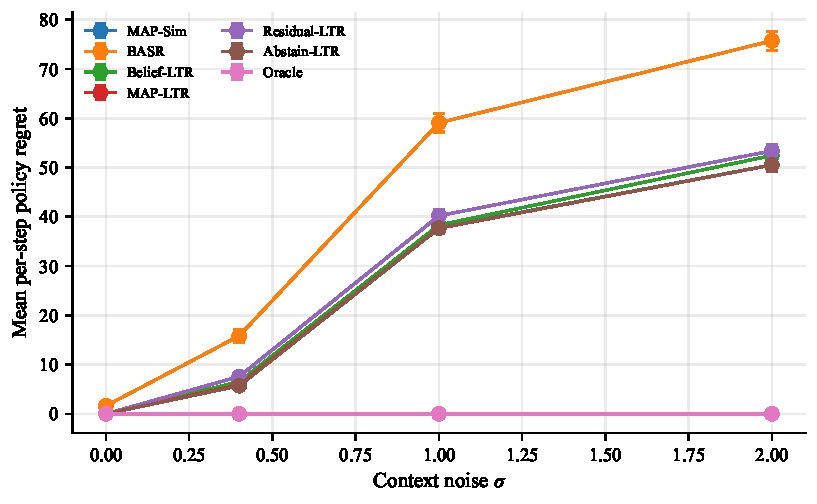
\includegraphics[width=\linewidth]{figures/regret_vs_sigma_full.pdf}
\caption{Mean per-step policy regret against context noise for all ranking operators. Error bars denote SEM across thirty seeds.}
\label{fig:regret}
\end{figure}

\begin{table}[t]
\centering
\caption{Regime map of mean per-step policy regret (mean \(\pm\) SD over thirty seeds).}
\label{tab:regime}
\scriptsize
\setlength{\tabcolsep}{3.0pt}
\begin{tabular}{@{}lcccc@{}}
\toprule
Operator & \(\sigma=0\) & \(\sigma=0.4\) & \(\sigma=1.0\) & \(\sigma=2.0\) \\
\midrule
MAP-Sim & \(0.00\pm0.00\) & \(6.18\pm3.15\) & \(37.77\pm5.88\) & \(50.54\pm7.33\) \\
BASR & \(1.61\pm0.49\) & \(15.82\pm7.34\) & \(59.08\pm10.18\) & \(75.73\pm10.32\) \\
Belief-LTR & \(0.00\pm0.00\) & \(6.51\pm3.51\) & \(38.32\pm7.30\) & \(52.45\pm7.65\) \\
MAP-LTR & \(0.00\pm0.00\) & \(5.88\pm3.08\) & \(37.68\pm5.90\) & \(50.52\pm7.32\) \\
Residual-LTR & \(0.00\pm0.00\) & \(7.56\pm3.11\) & \(40.21\pm6.51\) & \(53.40\pm7.30\) \\
Abstain-LTR & \(0.00\pm0.00\) & \(5.69\pm3.16\) & \(37.71\pm5.93\) & \(50.54\pm7.33\) \\
Oracle & \(0.00\pm0.00\) & \(0.00\pm0.00\) & \(0.00\pm0.00\) & \(0.00\pm0.00\) \\
\bottomrule
\end{tabular}
\end{table}

\begin{table}[t]
\centering
\caption{Belief-feature ablation at fixed model capacity (30 seeds). A positive difference indicates that soft belief features increase regret.}
\label{tab:ablation}
\footnotesize
\begin{tabular}{@{}lccc@{}}
\toprule
\(\sigma\) & Belief-LTR & MAP-LTR & Difference \\
\midrule
0.0 & \(0.00\) & \(0.00\) & \(0.00\) \\
0.4 & \(6.51\) & \(5.88\) & \(+0.63\) \\
1.0 & \(38.32\) & \(37.68\) & \(+0.64\) \\
2.0 & \(52.45\) & \(50.52\) & \(+1.93\) \\
\bottomrule
\end{tabular}
\end{table}

\subsection{Risk-Neutral Regime Map}
\label{sec:comparison}

Table~\ref{tab:regime} answers the risk-neutral part of the research question.
Regret increases by more than an order of magnitude between \(\sigma=0\) and \(\sigma=2\) for every feasible operator: among the variables we vary, context noise is the dominant factor.
Belief averaging is worse than belief collapse at every noise level; the paired MAP-Sim vs BASR delta at \(\sigma=2\) is \(+25.19\) (bootstrap \(95\%\) CI \([21.77,28.72]\), \(p\ll 10^{-10}\)).
The learned operators likewise fail to overturn belief collapse.
Residual correction is harmful at high noise, adding \(2.86\) regret units at \(\sigma=2\) relative to MAP-Sim.
Confidence-gated deferral is safe rather than transformative: it matches belief collapse at \(\sigma\in\{0,2\}\) and improves it only slightly at \(\sigma=0.4\).

Secondary metrics at \(\sigma=2\) (Table~\ref{tab:secondary}) reinforce the same picture.
Belief averaging is worse in regret and about five times slower than belief collapse.

\begin{table}[t]
\centering
\caption{Secondary metrics at \(\sigma=2\), averaged over thirty seeds.}
\label{tab:secondary}
\footnotesize
\begin{tabular}{@{}lccc@{}}
\toprule
Operator & Top-1 & Episode reward & Latency (ms) \\
\midrule
MAP-Sim & \(0.594\) & \(738.9\) & \(2.25\) \\
BASR & \(0.464\) & \(507.3\) & \(11.49\) \\
Belief-LTR & \(0.579\) & \(707.6\) & \(1.71\) \\
Abstain-LTR & \(0.594\) & \(738.9\) & \(5.43\) \\
Oracle & \(1.000\) & \(1768.5\) & \(1.99\) \\
\bottomrule
\end{tabular}
\end{table}

\subsection{Interpretation}
\label{sec:interpretation}

Under the myopic risk-neutral utility of~\eqref{eq:utility}, collapsed context is sufficient for the strongest observed risk-neutral performance among the operators we compare.
That reading motivates changing the aggregation functional rather than only the feature set.
The risk-sensitive study in Section~\ref{sec:cvar} tests that hypothesis.

\subsection{Risk-Sensitive Aggregation and Hybrid Gate}
\label{sec:cvar}

Keeping the interface of~\eqref{eq:operator} unchanged, we replace the risk-neutral aggregation with a tail-sensitive one~\cite{rockafellar2000cvar,chow2015cvar}.
We maximise the \emph{lower-tail} CVaR of utility, using the Rockafellar--Uryasev representation~\cite{rockafellar2000cvar} (equivalently, CVaR of the loss \(-U_t\)):
\begin{align}
\label{eq:cvar}
\mathrm{CVaR}_\alpha(a)
=\max_{\eta\in\mathbb{R}}\Biggl[\eta-\frac{1}{\alpha}\,\mathbb{E}_{c\sim p_t}\bigl[(\eta-U_t(a\mid c))_+\bigr]\Biggr]\:,
\end{align}
where \((\cdot)_+=\max\{\cdot,0\}\) and we select \(a_t=\arg\max_{a\in\mathcal{A}}\mathrm{CVaR}_\alpha(a)\) with \(\alpha=0.3\).
Because \(\mathcal{C}=\{0,1\}\) is binary,~\eqref{eq:cvar} reduces to a two-point tail mean: if the worse context already carries mass at least \(\alpha\), \(\mathrm{CVaR}_\alpha\) collapses to that worst-case utility (a minimax selector); only when the worse mass is below \(\alpha\) does it blend the two utilities.
That degeneracy is a feature of the binary geometry, not a hidden extra algorithm, and it is what makes the hybrid gate closed-form.

The candidate set of~\eqref{eq:actions} has a specialize-versus-robust geometry: a specialized prompt returns \(H\) in its matching context but only \(L\) in the mismatched one, whereas the robust prompt returns \(M\) in both.
Let \(\pi_t\) be the belief peak on the specialised prompt's matching context and write \(\varrho=(H-M)/(H-L)\).
Comparing \(\mathrm{CVaR}_\alpha\) of the specialised prompt with the constant score \(M\) of the robust prompt yields the crossover
\begin{align}
\label{eq:crossover}
\pi^\star(\alpha)=1-\alpha\varrho\:,
\end{align}
i.e.\ the robust prompt is preferred once \(\pi_t<\pi^\star\).
(The same algebra gives \(\pi^\star=1-\alpha\) in the pure-minimax regime \(\pi_t\le 1-\alpha\), which is stricter and is absorbed by~\eqref{eq:crossover} whenever \(\varrho\le 1\).)
We estimate \(H\), \(M\) and \(L\) as empirical means of the corresponding one-step utilities under the locked StepCountJITAI configuration used for the regime map, obtaining \(H\approx 51.45\), \(M\approx 12.94\) and \(L\approx 0.09\), hence \(\varrho\approx 0.75\) and a theory point estimate \(\pi^\star(\alpha)\approx 0.775\) at \(\alpha=0.3\).
Equation~\eqref{eq:crossover} is therefore a closed-form consequence of this H/M/L structure, not a universal law across arbitrary candidate geometries.
Within that structure it holds empirically as a decision rule: below \(\pi^\star\) the tail-sensitive operator selects the robust prompt on \(100\%\) of steps while disagreeing with belief collapse on \(93\%\) of them, whereas above \(\pi^\star\) the two rules almost never disagree.
A hybrid operator therefore applies belief collapse when \(\pi_t\ge\pi^\star\) and the tail-sensitive score otherwise.
We use the \emph{operational} gate \(\pi^\star=0.7\) selected on a held-out validation grid (Fig.~\ref{fig:pi-sweep}): at high \(\sigma\) it slightly improves on the theory point \(0.775\), while remaining close to pure CVaR where the gate opens.

Table~\ref{tab:cvar} reports the risk-sensitive study over the same thirty-seed protocol as Table~\ref{tab:regime} and confirms the prediction at high noise.
Tail-sensitive ranking reduces regret by \(16.76\) units at \(\sigma=1\) and by \(24.89\) units at \(\sigma=2\) (\(\approx 49\%\) relative to MAP's \(50.54\)).
Regret is measured in the simulator's one-step utility units (the same scale as \(H/M/L\)), not in physical step counts.
Paired bootstrap \(95\%\) intervals on the seed-wise delta (CVaR\(-\)MAP) are \([-18.91,-14.76]\) at \(\sigma=1\) and \([-27.57,-22.46]\) at \(\sigma=2\); both exclude zero (paired \(t\) \(p\ll 10^{-10}\)).
Hybrid shows the same qualitative pattern, with delta \(-26.09\) at \(\sigma=2\) (CI \([-28.72,-23.50]\)).
At low noise the ordering reverses, costing \(2.50\) units at \(\sigma=0\), because pessimism insures against contexts that carry almost no belief mass.
Gate usage follows the same pattern, with the tail-sensitive branch handling \(0.02\), \(0.15\), \(0.56\) and \(0.91\) of steps as \(\sigma\) rises through the grid under \(\pi^\star=0.7\).

\begin{figure}[t]
\centering
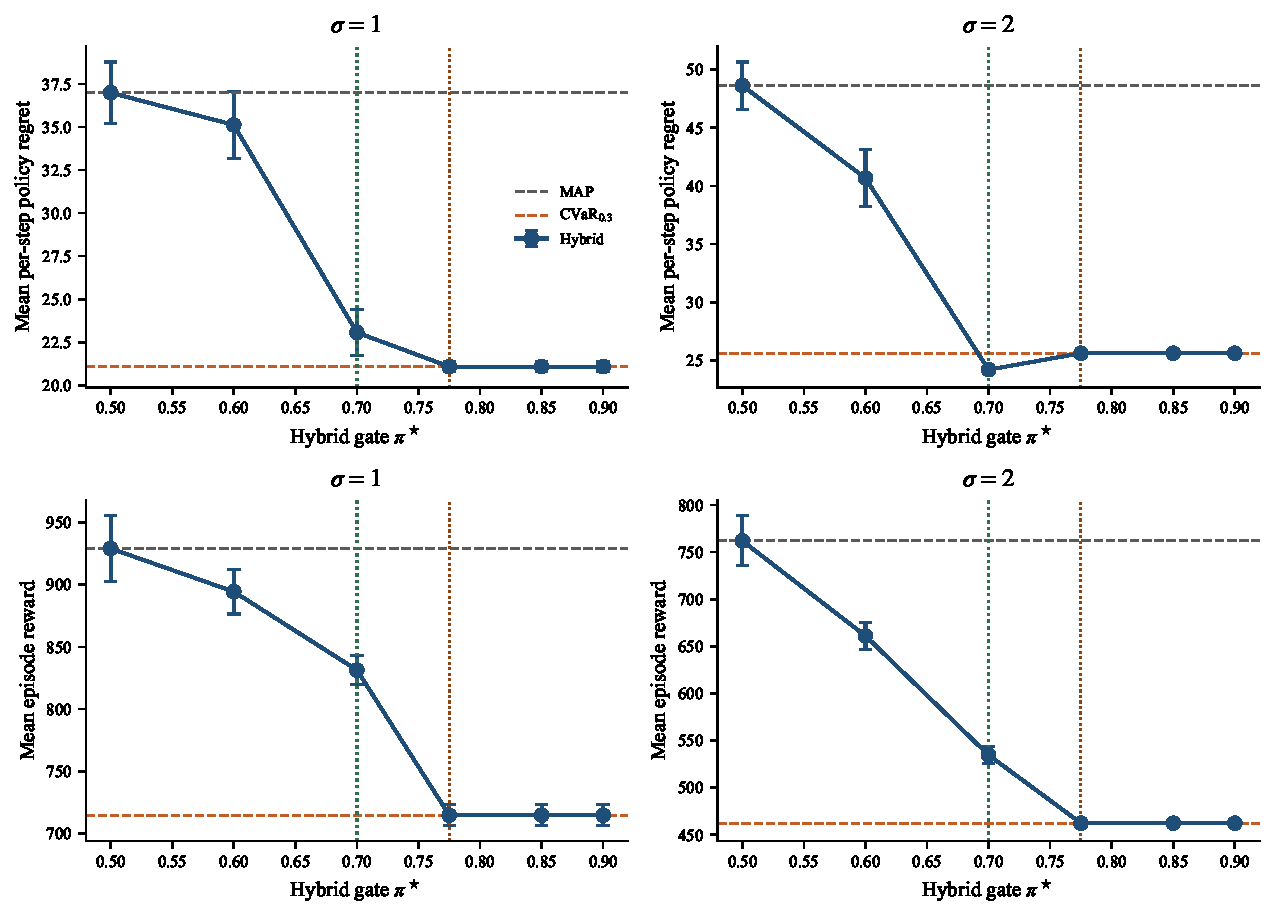
\includegraphics[width=\linewidth]{figures/pi_sweep_regret_reward.pdf}
\caption{Hybrid gate sweep: mean per-step regret (top) and mean episode reward (bottom) versus \(\pi^\star\) at \(\sigma\in\{1,2\}\) (12 seeds). Vertical lines mark the operational gate \(0.7\) and the theory estimate \(\approx 0.775\); dashed horizontals are MAP and CVaR\(_{0.3}\).}
\label{fig:pi-sweep}
\end{figure}

\begin{table}[t]
\centering
\caption{Risk-sensitive ranking on StepCountJITAI (mean \(\pm\) SEM, 30 seeds). Negative \(\Delta\) favours that operator over MAP.}
\label{tab:cvar}
\scriptsize
\setlength{\tabcolsep}{2.6pt}
\begin{tabular}{@{}lccccc@{}}
\toprule
\(\sigma\) & MAP & CVaR & Hybrid & \(\Delta\) CVaR & \(\Delta\) Hybrid \\
\midrule
0.0 & \(0.00\pm0.00\) & \(2.50\pm0.00\) & \(2.50\pm0.00\) & \(+2.50\) & \(+2.50\) \\
0.4 & \(6.18\pm0.57\) & \(8.13\pm0.14\) & \(7.90\pm0.31\) & \(+1.95\) & \(+1.72\) \\
1.0 & \(37.77\pm1.07\) & \(21.01\pm0.17\) & \(24.15\pm1.04\) & \(-16.76\) & \(-13.62\) \\
2.0 & \(50.54\pm1.34\) & \(25.65\pm0.02\) & \(24.45\pm0.13\) & \(-24.89\) & \(-26.09\) \\
\bottomrule
\end{tabular}
\end{table}

\begin{figure*}[!t]
\centering
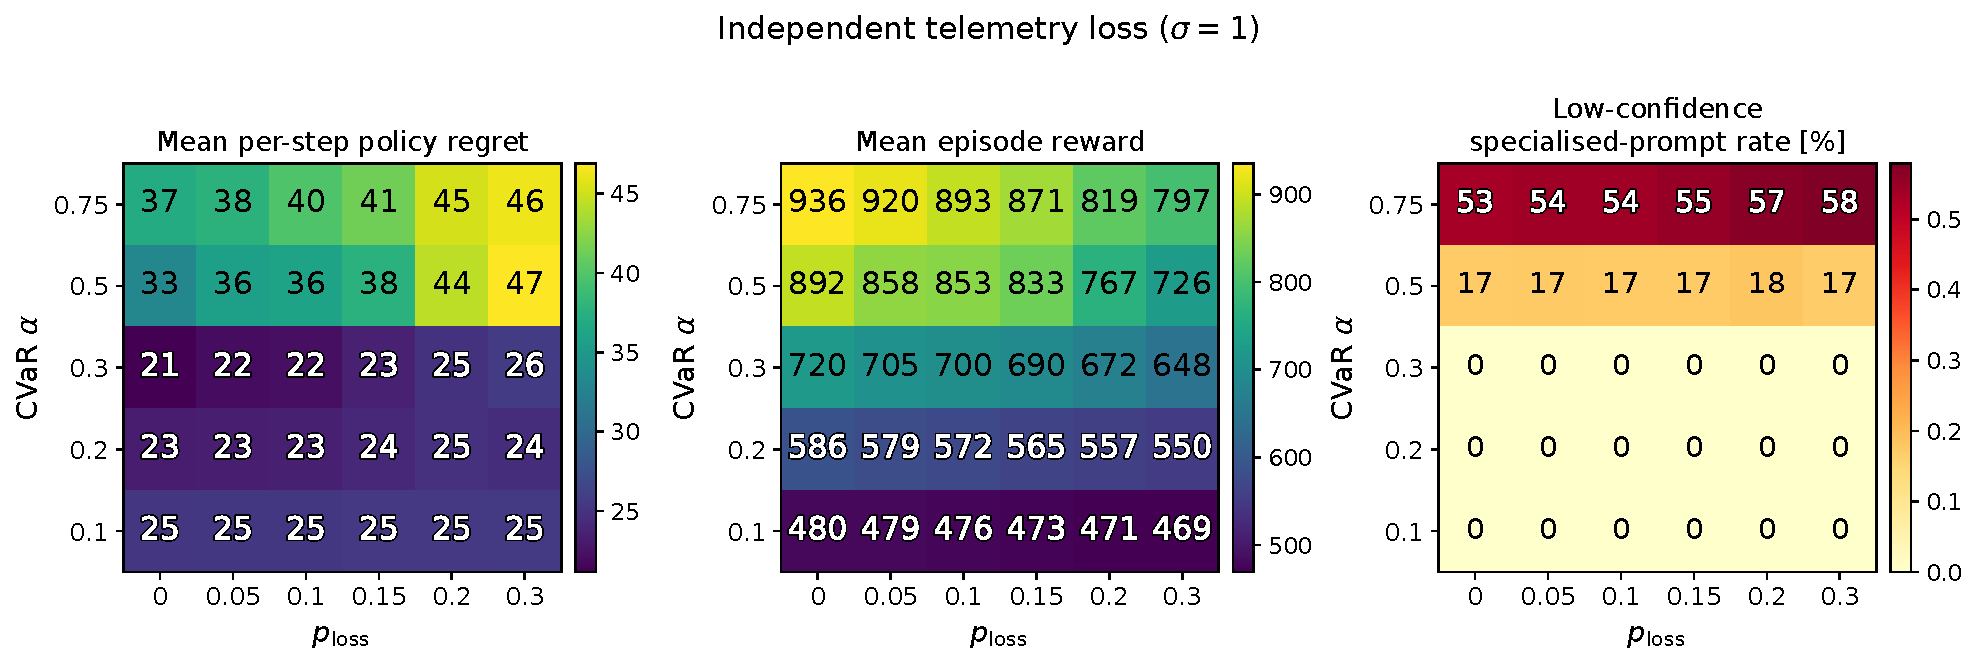
\includegraphics[width=\textwidth]{figures/heatmap_independent_alpha_ploss.pdf}\\[0.35em]
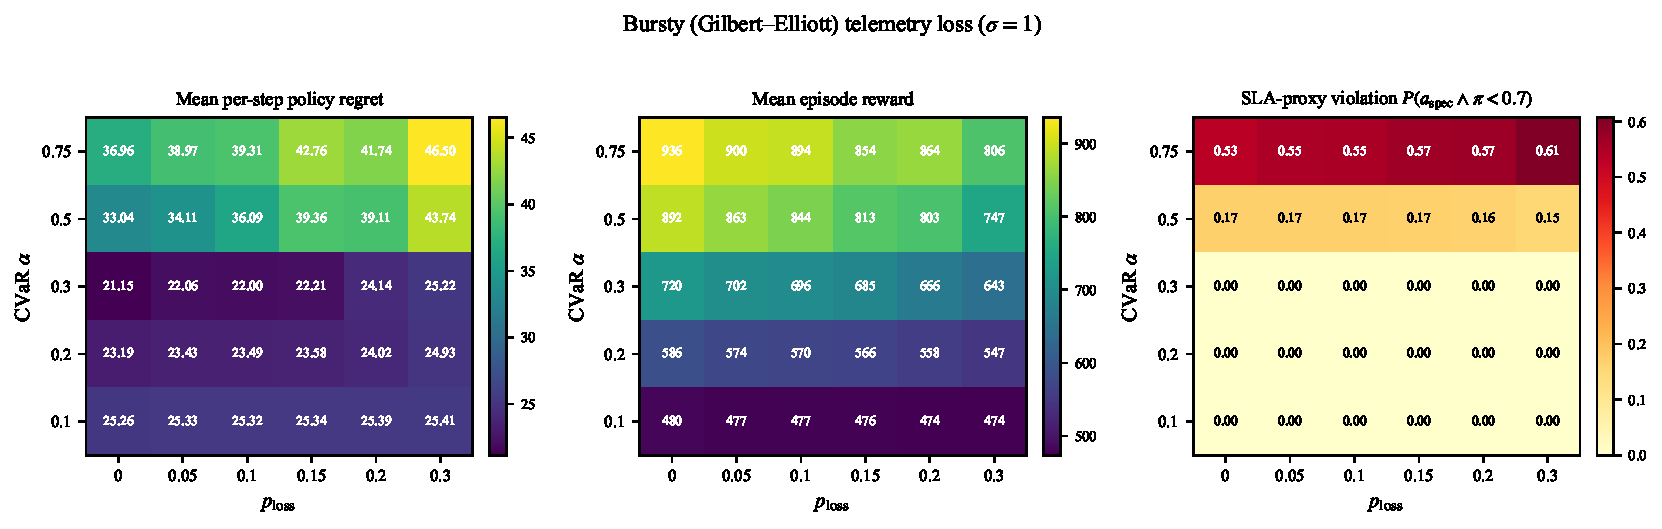
\includegraphics[width=\textwidth]{figures/heatmap_bursty_alpha_ploss.pdf}
\caption{Telemetry loss at \(\sigma=1\): independent (top) and bursty (bottom) CVaR heatmaps over \((\alpha,p_{\mathrm{loss}})\) for mean per-step regret, mean episode reward and SLA-proxy violation \(P(a_{\mathrm{spec}}\wedge\pi{<}0.7)\) (10 seeds).}
\label{fig:heatmap-sigma1}
\end{figure*}

\begin{figure*}[!t]
\centering
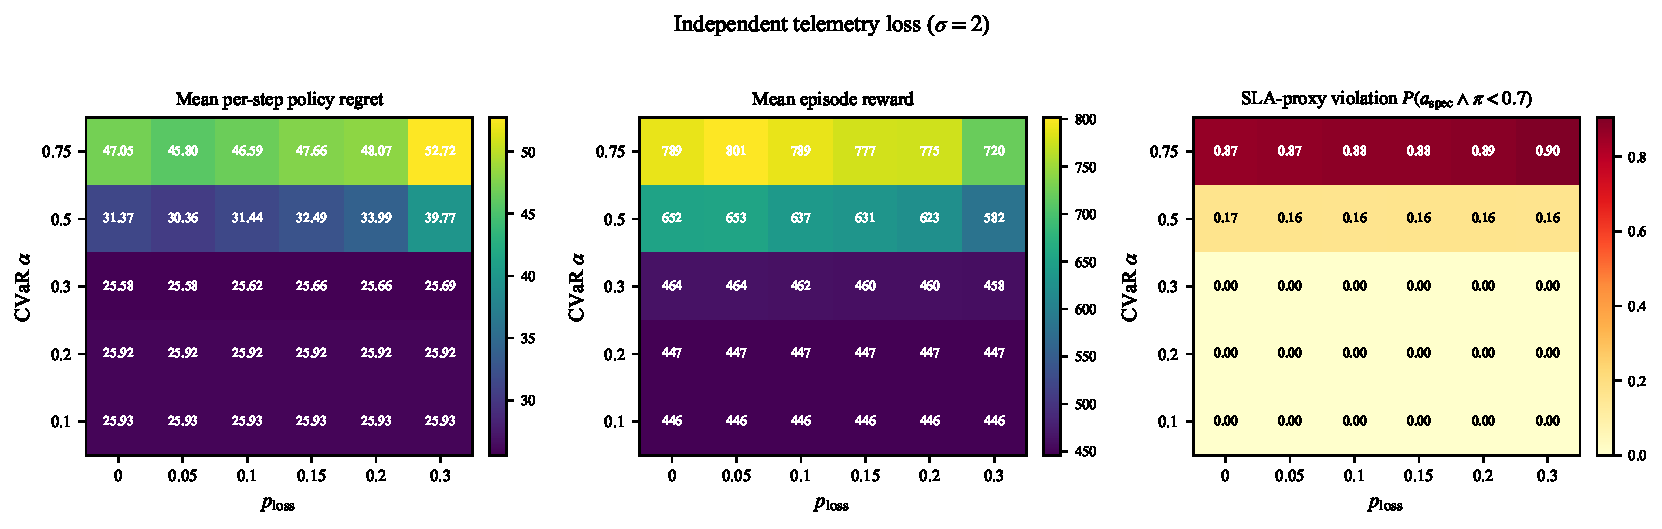
\includegraphics[width=\textwidth]{figures/heatmap_independent_alpha_ploss_sigma2.pdf}\\[0.35em]
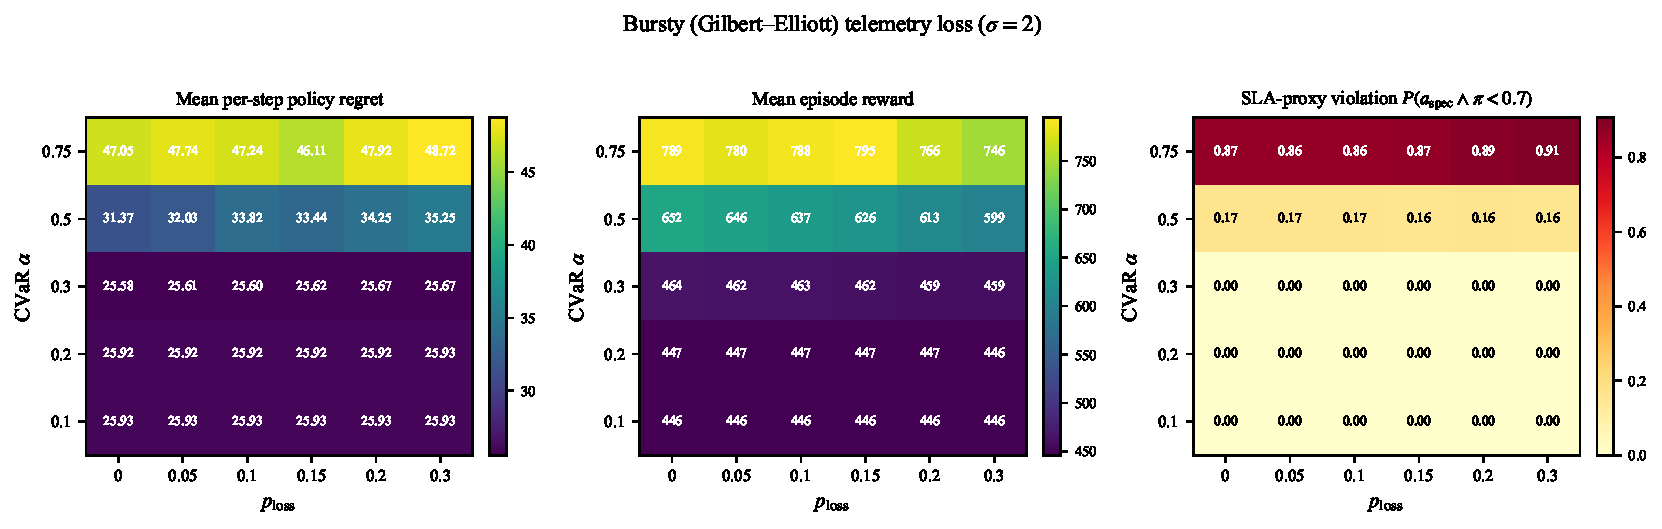
\includegraphics[width=\textwidth]{figures/heatmap_bursty_alpha_ploss_sigma2.pdf}
\caption{Telemetry loss at \(\sigma=2\): independent (top) and bursty (bottom) CVaR heatmaps over \((\alpha,p_{\mathrm{loss}})\), same metrics as Fig.~\ref{fig:heatmap-sigma1} (10 seeds).}
\label{fig:heatmap-sigma2}
\end{figure*}

\subsection{Mechanism: Decision Rule vs Episode Gain}
\label{sec:mechanism}

The scientifically central observation is a dissociation between decision accuracy and episode regret (Fig.~\ref{fig:twin}).
A calibrated one-step synthetic twin that reproduces the same utility geometry confirms the \(\pi^\star\) decision rule at \(99.6\%\) accuracy, yet the regret advantage does not appear there: the tail-sensitive operator is never better under pure one-step Bayes regret.
Consistent with this, the belief-collapse error stays below \(\varrho\) at every noise level, reaching only \(0.35\) at \(\sigma=2\).
The episode-level gain on StepCountJITAI is therefore consistent with trajectory mediation: safer prompts slow disengagement and shift the state distribution, rather than improving pure one-step Bayes regret.
By preferring the robust prompt when \(\pi_t\) is low, tail-sensitive selection avoids mismatched specialised prompts that inflate \(D_t\) and blunt future reward, so later decisions face a healthier habit / engagement trajectory even when the one-step Bayes gap is small.

We test that reading directly by freezing habituation and disengagement updates (\(\varepsilon_h=\delta_h=\varepsilon_d=\delta_d=0\), with \(D\)-termination disabled) while leaving belief noise unchanged (Table~\ref{tab:hd}).
Under baseline dynamics the CVaR\(-\)MAP delta remains about \(-16.3\) at \(\sigma=1\) and \(-24.4\) at \(\sigma=2\) (20 seeds).
Under frozen \(H/D\) the sign reverses to about \(+50.5\) and \(+61.7\): without trajectory coupling, tail-sensitive ranking is worse than MAP on the same one-step utility.
We confirmed the high-noise episode gain under stochastic dynamics (\(n_{\mathrm{version}}=1\)) and under a stronger process-noise transfer setting (Table~\ref{tab:lock}): at \(\sigma=2\), CVaR still reduces regret by about \(23\)--\(24\) units relative to MAP-Sim.
An alternate one-step geometry again fails to reproduce the episode-level gain, which is consistent with trajectory mediation and warns against treating \(\pi^\star\) as geometry-independent.

\begin{figure}[t]
\centering
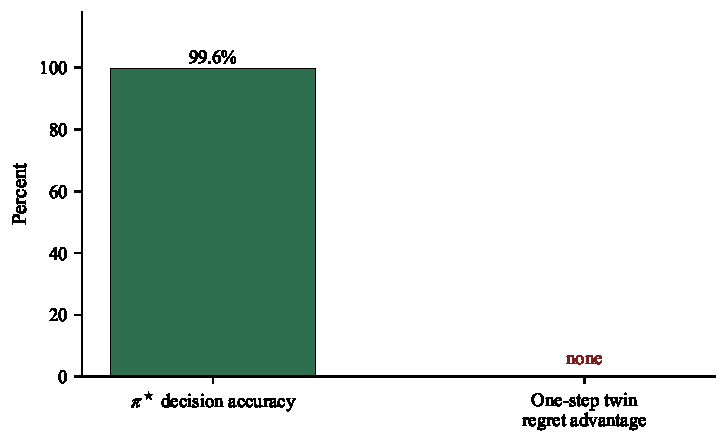
\includegraphics[width=0.92\linewidth]{figures/twin_dissociation.pdf}
\caption{On the calibrated one-step twin, \(\pi^\star\) is recovered as a decision rule, but the episode-style regret win does not appear.}
\label{fig:twin}
\end{figure}

\begin{table}[t]
\centering
\caption{H/D ablation: mean \(\Delta\) (CVaR\(-\)MAP) \(\pm\) SEM over 20 seeds.}
\label{tab:hd}
\footnotesize
\begin{tabular}{@{}lcc@{}}
\toprule
Condition & \(\sigma=1\) & \(\sigma=2\) \\
\midrule
Baseline dynamics & \(-16.32\pm1.16\) & \(-24.38\pm1.36\) \\
Frozen \(H/D\) & \(+50.53\pm0.55\) & \(+61.67\pm0.78\) \\
\bottomrule
\end{tabular}
\end{table}

\begin{table}[t]
\centering
\caption{Lock validation at \(\sigma=2\) (mean step regret). Negative \(\Delta\) favours CVaR.}
\label{tab:lock}
\footnotesize
\begin{tabular}{@{}lcc@{}}
\toprule
Setting & MAP & \(\Delta\) CVaR \\
\midrule
Stochastic (\(n{=}1\), \(\sigma_s{=}10\), 15 seeds) & \(49.52\) & \(-23.78\) \\
Transfer (\(\sigma_s{=}20\), 15 seeds) & \(49.33\) & \(-22.86\) \\
\bottomrule
\end{tabular}
\end{table}

\subsection{Deployable Proxy, Telemetry Loss Heatmaps and SLA Reading}
\label{sec:proxy}

Oracle regret is a research instrument.
For service operation we also report a deployable proxy that needs no true context: the rate of specialised prompts issued when the belief peak is below \(0.7\) (Table~\ref{tab:proxy}).
We reuse the same event as an \emph{SLA-proxy violation} under impaired telemetry: \(P(a_t\in\{2,3\}\wedge\pi_t{<}0.7)\) evaluated on the belief actually consumed by the ranker.
At \(\sigma=2\), MAP-Sim issues such low-confidence specialised prompts on \(89.2\%\) of steps, whereas CVaR drives that rate to \(0.0\%\) by shifting mass to the robust prompt (\(75.3\%\) robust vs \(0.0\%\) for MAP).

\paragraph{Independent and bursty packet loss.}
We sweep mean loss \(p_{\mathrm{loss}}\in\{0,0.05,0.10,0.15,0.20,0.30\}\) under both channels at \(\sigma\in\{1,2\}\) (10 seeds, 10 episodes per cell), crossed with \(\alpha\in\{0.1,0.2,0.3,0.5,0.75\}\).
This secondary grid uses fewer seeds and episodes than the primary 30-seed study, so its \(p_{\mathrm{loss}}=0\) sample means need not match Table~\ref{tab:cvar}; all loss contrasts are made within matched cells.
Fig.~\ref{fig:heatmap-sigma1} shows the \(\sigma=1\) heatmaps; Fig.~\ref{fig:heatmap-sigma2} shows the corresponding \(\sigma=2\) grids for both channels.
Across both noise levels, \(\alpha\approx 0.3\) remains the best operating region: \(\alpha=0.1\) pays an insurance premium, while \(\alpha\ge 0.5\) approaches risk-neutral behaviour.
Table~\ref{tab:loss} summarises the \(\alpha=0.3\) slice.
At \(\sigma=1\) and \(p_{\mathrm{loss}}=0.20\), independent loss gives MAP \(45.2\) vs CVaR \(24.9\) (\(\Delta\approx -20.4\)); bursty gives \(41.7\) vs \(24.1\) (\(\Delta\approx -17.6\)).
At \(\sigma=2\) the advantage widens: independent \(\Delta\approx -22.4\) at \(20\%\) loss and \(\Delta\approx -27.0\) at \(30\%\); bursty deltas stay near \(-21\) to \(-23\).
CVaR's SLA-proxy violation remains \(0.00\) on every cell, while MAP's rises from about \(0.53\)--\(0.61\) at \(\sigma=1\) to \(0.86\)--\(0.91\) at \(\sigma=2\).
Risk-sensitive ranking therefore remains preferable under i.i.d.\ and bursty monitoring drops at matched mean loss.

Table~\ref{tab:sla} summarises service-facing latency under SLA-style targets (multi-tenant cells: mean \(\pm\) SD over \(8\) desktop repeats).
Single-decision ranking p50 stays near \(1\)\,ms for MAP and CVaR; a Poisson arrival model at \(\lambda=100\)\,s\(^{-1}\) with four workers keeps sojourn p95 near \(3.2\)\,ms for both.
Multi-tenant concurrent twin+rank load is pushed from \(8\) to \(32\) and \(64\) users: p95 rises with concurrency for both methods.
Bootstrap \(95\%\) CIs on the CVaR$-$MAP p95 difference (over the eight repeats) include zero at \(N{=}8\) and \(N{=}32\), so the apparent mid-scale crossover is not distinguishable from scheduling noise; at \(N{=}64\) the CI excludes zero (about \(+16\)\,ms mean, favouring MAP on latency) while throughput remains hundreds of decisions/s for both.
Non-monotonic mean throughput across \(N\) stays within the reported run-to-run SD bands in Table~\ref{tab:sla}.
Thus CVaR's regret reduction of about \(24.9\) units at \(\sigma=2\) does not buy a material ranking-stage penalty at modest concurrency; at higher tenant counts a modest latency cost appears, still secondary to the regret / proxy win for operators whose ranking budgets are already on the order of tens of milliseconds~\cite{shi2016edge}.

\begin{table}[t]
\centering
\caption{Deployable proxy at high noise (20 seeds).}
\label{tab:proxy}
\footnotesize
\begin{tabular}{@{}lcccc@{}}
\toprule
Method & \(\sigma\) & Spec.\ rate & Low-conf.\ spec. & Robust rate \\
\midrule
MAP-Sim & 1.0 & \(0.957\) & \(0.553\) & \(0.000\) \\
CVaR\(_{0.3}\) & 1.0 & \(0.200\) & \(0.000\) & \(0.566\) \\
MAP-Sim & 2.0 & \(0.988\) & \(0.892\) & \(0.000\) \\
CVaR\(_{0.3}\) & 2.0 & \(0.012\) & \(0.000\) & \(0.753\) \\
\bottomrule
\end{tabular}
\end{table}

\begin{table}[t]
\centering
\caption{Telemetry loss at \(\alpha=0.3\) (10 seeds; mean step regret). Independent (iid) vs bursty (b) channels at matched mean \(p_{\mathrm{loss}}\), for \(\sigma\in\{1,2\}\).}
\label{tab:loss}
\scriptsize
\setlength{\tabcolsep}{2.4pt}
\resizebox{\columnwidth}{!}{%
\begin{tabular}{@{}lcccccccc@{}}
\toprule
 & \multicolumn{4}{c}{\(\sigma=1\)} & \multicolumn{4}{c}{\(\sigma=2\)} \\
\cmidrule(lr){2-5}\cmidrule(lr){6-9}
\(p_{\mathrm{loss}}\) & M\(_{\mathrm{iid}}\) & C\(_{\mathrm{iid}}\) & M\(_{\mathrm{b}}\) & C\(_{\mathrm{b}}\) & M\(_{\mathrm{iid}}\) & C\(_{\mathrm{iid}}\) & M\(_{\mathrm{b}}\) & C\(_{\mathrm{b}}\) \\
\midrule
\(0\%\) & \(37.0\) & \(21.2\) & \(37.0\) & \(21.2\) & \(47.1\) & \(25.6\) & \(47.1\) & \(25.6\) \\
\(5\%\) & \(37.7\) & \(22.0\) & \(39.0\) & \(22.1\) & \(45.8\) & \(25.6\) & \(47.7\) & \(25.6\) \\
\(10\%\) & \(39.9\) & \(22.2\) & \(39.3\) & \(22.0\) & \(46.6\) & \(25.6\) & \(47.2\) & \(25.6\) \\
\(15\%\) & \(41.3\) & \(23.5\) & \(42.8\) & \(22.2\) & \(47.7\) & \(25.7\) & \(46.1\) & \(25.6\) \\
\(20\%\) & \(45.2\) & \(24.9\) & \(41.7\) & \(24.1\) & \(48.1\) & \(25.7\) & \(47.9\) & \(25.7\) \\
\(30\%\) & \(46.2\) & \(25.7\) & \(46.5\) & \(25.2\) & \(52.7\) & \(25.7\) & \(48.7\) & \(25.7\) \\
\bottomrule
\end{tabular}}
\\[0.2em]
{\scriptsize M\,=\,MAP, C\,=\,CVaR\(_{0.3}\).}
\end{table}

\begin{table}[t]
\centering
\caption{SLA-style ranking-stage feasibility (desktop). Multi-tenant cells: mean\(\pm\)SD over \(8\) repeats.}
\label{tab:sla}
\scriptsize
\setlength{\tabcolsep}{3.2pt}
\begin{tabular}{@{}lccc@{}}
\toprule
Setting & MAP & CVaR\(_{0.3}\) & Notes \\
\midrule
Rank p50 (ms) & \(1.02\) & \(1.08\) & single run \\
Sojourn p95 (ms) & \(3.2\) & \(3.2\) & \(\lambda{=}100\)/s, 4 wrk. \\
8-user p95 (ms) & \(21.6\pm2.2\) & \(21.6\pm2.0\) & \(470\pm29\) / \(466\pm19\)/s \\
32-user p95 (ms) & \(103\pm27\) & \(92\pm12\) & \(421\pm63\) / \(459\pm23\)/s \\
64-user p95 (ms) & \(185\pm12\) & \(201\pm10\) & \(439\pm21\) / \(415\pm16\)/s \\
\bottomrule
\end{tabular}
\end{table}

%--------------------------------------------------------------------------
\section{Discussion}
\label{sec:discussion}

\subsection{Why Soft Belief Fails under Risk-Neutral Ranking}
On the ranking interface studied here, soft belief features and belief averaging do not beat MAP collapse under a shared one-step risk-neutral utility.
This does not contradict Karine et~al.~\cite{karine2023uai} for trained RL policies; it shows that the soft-belief advantage need not transfer to this explicit ranking setting.

\subsection{Geometry-Specific Reading of \texorpdfstring{\(\pi^\star\)}{pi*}}
The crossover \(\pi^\star(\alpha)=1-\alpha\varrho\) follows from the H/M/L utility structure of this candidate set.
It is a useful decision rule inside that geometry and should not be read as a universal ranking law.
The alternate one-step geometry that fails to reproduce the episode gain underscores that point.

\subsection{Scope of Systems Evidence}
\label{sec:scope}
Counterfactual oracle utility via environment snapshot/restore is not available in a live AIoT loop, where true context is never observed even post hoc.
Hence \(\mathcal{R}(\rho)\) is a research instrument for comparing ranking rules; the low-confidence specialised-prompt rate is the corresponding deployable proxy.
The scientific contribution is ranking under controlled monitoring impairment (\(\sigma\) and matched-mean independent / Gilbert--Elliott loss); systems packaging is secondary evidence for that claim.
Desktop multi-tenant benches measure ranking-stage latency and throughput on one host under thread-pool concurrency (Table~\ref{tab:sla})---they characterise the Rank module's compute envelope, not a multi-rack Kubernetes deployment.
The packet-loss channels stale the delivered belief at a prescribed mean \(p_{\mathrm{loss}}\), with independent and bursty variants matched on that mean so that burstiness is not confounded with a higher average drop rate.
As gateway plumbing evidence, a lab ESP32 published \(1\)\,Hz JSON telemetry over Wi‑Fi/MQTT to a desktop ranking bridge in two sequential sessions (MAP then CVaR; same device and broker, bridge restarted between rankers): \(212\) MAP and \(237\) CVaR logged decisions over about \(3.5\) and \(4.0\) minutes respectively (median RSSI near \(-63\)\,dBm).
The unequal counts reflect slightly longer CVaR wall time, not concurrent dual-ranker logging.
Replaying those records yields ranking-stage p95 latency of \(0.75\)\,ms (MAP) and \(1.51\)\,ms (CVaR)---consistent with the desktop microbench and well below the \(1\)\,s publish period.
On-device step/HR sensing remains simulated in that lab loop; the ESP32 result is connectivity and ranking-stage timing only.

\subsection{Implications for Network and Service Management}
The practical takeaway for operators of closed-loop AIoT intervention services is modular: keep Sense--Monitor--Plan--Safety--Deliver fixed and treat Rank as the only policy surface under unreliable telemetry.
Risk-neutral soft belief is not a free upgrade on this interface; when monitoring reliability is poor (high \(\sigma\) or packet loss), risk-sensitive aggregation (CVaR / Hybrid with \(\pi^\star=0.7\)) is the change that moves both research regret and the deployable specialised-prompt / SLA proxy, with only a modest ranking-stage latency trade-off appearing at high concurrent tenant counts in our benches.
Because the episode gain is trajectory-mediated, service KPIs should track engagement / habituation-sensitive outcomes over windows longer than one decision, not only one-step accuracy.

%--------------------------------------------------------------------------
\section{Conclusion}
\label{sec:conclusion}

Under the ranking interface studied here, risk-neutral soft belief and LTR do not automatically beat MAP as context noise grows on StepCountJITAI~\cite{karine2023uai,karine2024stepcount}.
Changing aggregation to CVaR / Hybrid reverses the high-noise ordering: CVaR cuts regret by \(24.89\) units at \(\sigma=2\) and Hybrid (\(\pi^\star=0.7\)) by \(26.09\) (30 seeds; bootstrap CIs exclude zero), with gains preserved under stochastic dynamics, stronger process noise and independent / bursty packet-loss heatmaps at \(\sigma\in\{1,2\}\).
Evidence from a calibrated synthetic twin and from an \(H/D\) freeze ablation is consistent with trajectory mediation of the episode gain and with a geometry-specific reading of \(\pi^\star\).
A deployable proxy KPI, multi-tenant ranking-latency benches and a lab ESP32 / MQTT gateway loop connect the ranking module to managed AIoT service operation.
Future work includes long-horizon service objectives beyond mean per-step policy regret, additional utility geometries and multi-user contention under richer transport traces.

%--------------------------------------------------------------------------
\bibliographystyle{IEEEtran}
\bibliography{references}

\end{document}
